\section{实验二\ 内核引导启动}

\subsection{实验目的}

\begin{enumerate}
    \item 掌握系统中断的调用。
    \item 熟悉 system 加载的过程。
    \item 熟悉 GDTR 与 IDTR 的设置。
    \item 了解全局描述符格式。
    \item 了解由实模式到保护模式的跳转过程。
\end{enumerate}

\subsection{BIOS 启动过程}

计算机加电后,并非直接执行操作系统,而是执行系统初始化软件,完成基本 I/O 初始化和引导加载功能。

以 Intel 80386 为例,该初始化软件就是基本输入输出系统(Basic Input Output System,BIOS),它存储在一个只读存储器(ROM)中。计算机加电后,CPU 从物理地址 0xFFFFFFF0(4G地址的顶端)开始执行。在 0xFFFFFFF0 处只存放了一条跳转指令,通过该指令跳到 BIOS 例行程序起始点。

BIOS 在执行硬件自检和初始化后,会选择一个启动设备(如软盘、硬盘、光盘等),并读取该设备的第一扇区(即主引导扇区或启动扇区)到内存的特定地址 0x7c00 处,然后 CPU 控制权会转移到该地址继续执行。

\subsection{引导扇区}

引导扇区(boot sector)可分为主引导扇区(MBR)和分区引导扇区(DBR)。\textbf{主引导扇区}\footnote{\url{https://en.wikipedia.org/wiki/Master_boot_record}}是磁盘的 0 柱面 0 磁头 1 扇区,大小为 512 字节。该扇区可被 BIOS 识别为引导扇区的条件是其第 510 和第 511 字节分别为 0x55 和 0xAA。在启动时,BIOS 会将该扇区装入内存的特定位置,并使 CS:IP (代码段寄存器和指令指针寄存器)指向此处,执行引导扇区的代码。

我们可以利用引导扇区,在没有操作系统的情况下,开机后直接执行我们编写的代码。而操作系统中最先被执行的代码,就是下文将提到的 bootsect.s.

\subsection{内核引导启动程序}

NEUOS 的内核引导启动程序位于 exp2/boot 目录下,主要包含以下文件。

\begin{itemize}
    \item bootsect.s 磁盘引导块程序,驻留在引导扇区中。在计算机接通电源,ROM BIOS 自检后,引导扇区中的内容由 BIOS 加载到内存 0x7C00 处。
    \item setup.s 主要作用是利用 ROM BIOS 中断读取机器系统数据,并将这些程序保存到 0x90000 开始的位置,即覆盖了 bootsect 程序所在的内存。由于 bootsect.s 已执行完毕,数据的保存不会影响程序正常运行。读取的数据如表 \ref{tab:setup程序读取并保留的参数} 所示。另外,setup 程序将 system 模块从以 0x1000:0000 开始的位置整块向下移动到 0x0000:0000 处,并加载中断描述符表寄存器 IDTR 和全局描述符表寄存器 GDTR,设置 2 个 GDT 描述符,开启 A20 地址线,并重写中断控制芯片 8259A(本次实验未涉及),将控制寄存器 CR0 第 0 比特位置为 1,从而进入 32 位保护模式。 
    \item binary.s 进入保护模式后运行的程序,它将打印一行字符串来显示工作状态。
\end{itemize}

\begin{table}[]
\caption{setup 程序读取并保留的参数}
\label{tab:setup程序读取并保留的参数}
\begin{tabular}{llll}
内存地址 & 长度 & 名称 & 描述 \\
0x90000 & 2B & 光标位置 & 列号(0x00-最左端),行号(0x00-最顶端) \\
0x90002 & 2B & 扩展内存数 & 系统从 1 MB 开始的扩展内存数值(KB) \\
0x90004 & 2B & 显示页面 & 当前显示页面 \\
0x90006 & 1B & 显示模式 &  \\
0x90007 & 1B & 字符列数 &  \\
0x90008 & 2B & ?? &  \\
0x9000A & 1B & 显示内存 & 显示内存(0x00-64k, 0x01-128, 0x02-192k, 0x03-256k) \\
0x9000B & 1B & 显示状态 & 0x00-彩色, I/O=0x3dX;0x01-单色, I/O=0x3bX \\
0x9000C & 2B & 特性参数 & 显示卡特性参数 \\
…… &  &  &  \\
0x90080 & 16B & 硬盘参数表 & 第 1 个硬盘的参数表 \\
0x90090 & 16B & 硬盘参数表 & 第 2 个硬盘的参数表(如果没有,则清零) \\
…… &  &  &  \\
0x901FC & 2B & 根设备号 & 根文件系统所在的设备号(bootsect.s 中设置)
\end{tabular}
\end{table}

\begin{mdframed}[hidealllines=true,backgroundcolor=gray!20]
\textbf{练习 }read\_it 子程序在 exp2/bootsect.s 中,用于快速读取软盘中内容。认真阅读此段代码和注释,包括其中的 read\_track 子程序。

尝试在报告中以流程图或伪代码等形式描述程序。请注意格式规范,逻辑正确。
\end{mdframed}

\begin{mdframed}[hidealllines=true,backgroundcolor=gray!20]
\textbf{练习 }尝试在 exp2/setup.s 文件中分别找到开启保护模式、设置 GDTR 的相关代码,并简要解释相关代码。
\end{mdframed}

\begin{mdframed}[hidealllines=true,backgroundcolor=gray!20]
\textbf{练习 }全局描述符表(GDT)在 exp2/setup.s 的 gdt 标号后定义。请阅读 2 个 GDT 的定义,给出其基地址、段限长、type 类别,并阐述得出答案的具体依据。详细信息可参考 Intel® 64 and IA-32 Architectures Software Developer’s Manual \footnote{\url{https://software.intel.com/sites/default/files/managed/39/c5/325462-sdm-vol-1-2abcd-3abcd.pdf}}第 2756 页。

GDT 格式如图 \ref{fig:GDT格式} 所示,由图可见 1 个 GDT 长度为 64 比特位,需要一个 16 位的十六进制数表示。其中,TYPE 类型如表 \ref{tab:数据段 TYPE}、表 \ref{tab:代码段 TYPE} 所示。请思考,Intel x86 架构采用的是大端模式还是小端模式?
\end{mdframed}

\begin{figure}[htbp]
    \centering
    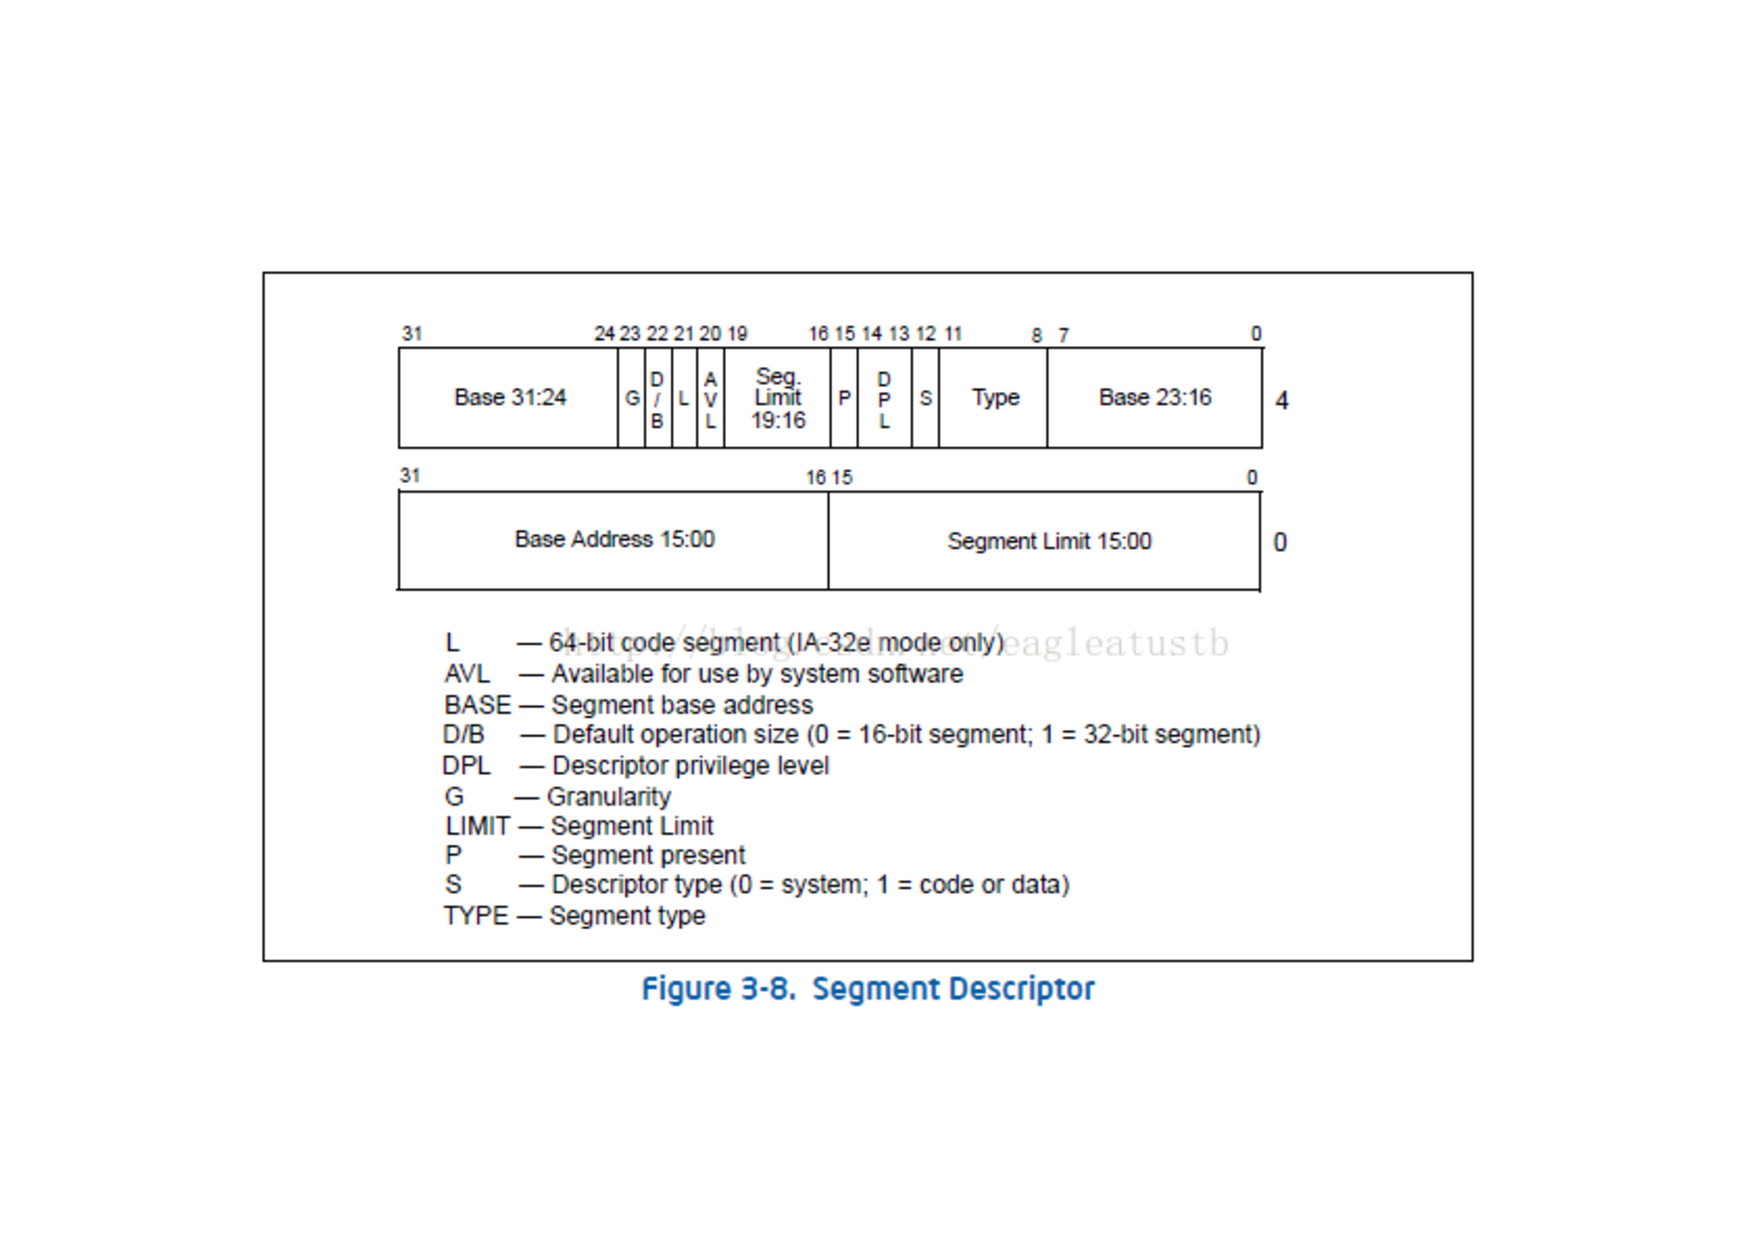
\includegraphics[width=\textwidth]{img/GDT格式.pdf}
    \caption{GDT 格式}
    \label{fig:GDT格式}
\end{figure}

\begin{table}[]
\caption{数据段 TYPE}
\label{tab:数据段 TYPE}
\begin{tabular}{llllll}
 & TYPE & 说明 &  &  &  \\
十进制值 &  & E & W & A & 数据段 \\
0 & 0 & 0 & 0 & 0 & 只读 \\
1 & 0 & 0 & 0 & 1 & 只读、已访问 \\
2 & 0 & 0 & 1 & 0 & 读写 \\
3 & 0 & 0 & 1 & 1 & 读写、已访问 \\
4 & 0 & 1 & 0 & 0 & 只读、向下扩展 \\
5 & 0 & 1 & 0 & 1 & 只读、向下扩展、已访问 \\
6 & 0 & 1 & 1 & 0 & 读写、向下扩展 \\
7 & 0 & 1 & 1 & 1 & 读写、向下扩展、已访问
\end{tabular}
\end{table}

\begin{table}[]
\caption{代码段 TYPE}
\label{tab:代码段 TYPE}
\begin{tabular}{llllll}
 & TYPE & 说明 &  &  &  \\
十进制值 &  & C & R & A & 代码段 \\
8 & 1 & 0 & 0 & 0 & 只执行 \\
9 & 1 & 0 & 0 & 1 & 只执行、已访问 \\
10 & 1 & 0 & 1 & 0 & 执行、可读 \\
11 & 1 & 0 & 1 & 1 & 执行、可读、已访问 \\
12 & 1 & 1 & 0 & 0 & 只执行、一致 \\
13 & 1 & 1 & 0 & 1 & 只执行、一致、已访问 \\
14 & 1 & 1 & 1 & 0 & 执行、可读、一致 \\
15 & 1 & 1 & 1 & 1 & 执行、可读、一致、已访问
\end{tabular}
\end{table}

\subsection{BIOS 写字符中断}

\textit{BIOS 中断}是 BIOS 提供的中断服务,注意与操作系统提供的\textit{系统中断}相区别。系统中断调用的操作系统定义的中断服务程序,与 BIOS 没有直接联系。

写字符中断的信息如下。\footnote{\url{https://en.wikipedia.org/wiki/INT_10H}}\footnote{Color: \url{https://en.wikipedia.org/wiki/BIOS_Color_Attributes}}

\begin{lstlisting}
int 10h (AH = 13h) Write String
AL = Write mode
BH = Page Number
BL = Color 
CX = String length
DH = Row
DL = Column
ES:BP = Offset of string
\end{lstlisting}

\begin{mdframed}[hidealllines=true,backgroundcolor=gray!20]
\textbf{练习 }下面是 exp2/bootsect.s 中一段调用 BIOS 写字符中断 int 10h (AH = 13h) 的 AT\&T 汇编代码。请阅读这段代码,尝试具体解释这段代码如何实现了 int 10h。

\begin{lstlisting}
print_msg:
	mov	$0x03, %ah
	xor	%bh, %bh
	int	$0x10
	
	mov	$20, %cx
	mov	$0x0007, %bx	
	mov $msg1, %bp
	mov	$0x1301, %ax
	int	$0x10
\end{lstlisting}

\end{mdframed}

\subsection{bootsect 源码汇编、链接过程}

使编写好的汇编源码 bootsect.s 在模拟器上运行,需要用到 as、ld、objcopy 三个程序。其基本过程如下,bootsect.s 经 as 汇编后生成目标文件 bootsect.o; ld 将 bootsect.o 链接后生成 ELF 格式文件,链接时,ld 会默认给代码加上 0x08048000 的偏移值,我们需要让这个偏移值变为0,可通过 -Ttext 参数设置偏移值;最后 objcopy 将链接生成的 ELF 格式文件处理为 QEMU/bochs 可读取的 BIN 格式。

在此我们需要了解 BIN 格式与 ELF 格式文件的不同。

BIN 格式即 raw binary,这种文件只包含机器码;ELF 格式除了机器码外,还包含其他信息,诸如段(section)的加载地址,运行地址,重定位表,符号表等。

ELF 格式即可执行可链接格式 (Executable and Linkable Format),这种格式文件的体积比对应的BIN格式要大。

前述的汇编出的.o文件是 ELF 格式的文件,而此处我们需要让QEMU使用BIN格式的镜像。

关于上述操作使用的 as、ld、objcopy 详细参数,可在 neu-os 目录下的 Makefile 中查看。

\subsection{实模式}

在引导程序接替 BIOS 后,计算机处于实模式(16位)运行状态,在这种状态下软件可访问的物理内存空间在 1MB 以内,且不支持分页机制。

实模式是不安全的。实模式下数据和代码位于内存不同区域,操作系统并没有区别对待二者,且每一个指针都指向实际的物理地址。用户程序的指针有能力指向操作系统区域,甚至修改其内容。

实模式下逻辑地址转换到物理地址的方式是:将逻辑地址的段(segment)左移4位,然后加上逻辑地址中的偏移(offset),即得到物理地址。实模式下,多个逻辑地址可能被映射到同一物理地址。

为什么 16 位实模式仍然存在?为了向下兼容,而向下兼容也是有利有弊的。

\subsection{保护模式}

在保护模式下,80386 的全部 32 根地址线才有效,可寻址 4GB 的线性地址空间和物理地址空间,可访问 64TB 的逻辑地址空间,可采用分段存储管理机制和分页存储管理机制;保护模式下的特权级机制,在实现资源共享的同时保证代码数据的安全及任务的隔离。

\subsection{段式存储管理机制}

在保护模式下才能使用分段机制。分段机制将内存划分为段(segment),每个段有起始地址和长度限制。代码段、数据段所指的段与这个段是同一含义。

分段机制所需的数据结构是\textbf{段描述符}和\textbf{段描述符表};需要的参数是逻辑地址,它由\textbf{段选择子}(selector)和\textbf{段偏移}(offset)组成。

分段机制能将逻辑地址通过查表转换到线性地址,过程是:CPU 将逻辑地址中的段选择子的内容作为段描述符表的索引,找到表中对应的段描述符,然后将段描述符中保存的段基址加上逻辑地址中的段偏移值,形成线性地址。若不启动分页机制,线性地址等同于物理地址。

这一转换过程对于应用程序员来说是不可见的。线性地址长度为 32 位,线性地址空间容量为 4GB。

\textbf{全局描述符表}是一个保存多个段描述符的“数组”,其起始地址保存在全局描述符表寄存器GDTR中。GDTR 长 48 位,其中高 32 位为基地址,低 16 位为段界限。GDT 不能由 GDT 自身以内的描述符进行描述,因此处理器将 GDTR 寄存器作为 GDT 的特殊系统段。注意,全局描述符表第一个段描述符是空的。

\begin{mdframed}[hidealllines=true,backgroundcolor=gray!20]
\textbf{练习 }阅读本实验已编写好的 Makefile 文件,在读懂其中指令的基础上,结合实验一所学,通过 Bochs 运行编写好的程序。

使用 Bochs 顶部的 View 菜单中查看 GDT 的功能,保存运行截图如图 \ref{fig:Bochs查看GDT} 所示。

\end{mdframed}

\begin{figure}[htbp]
    \centering
    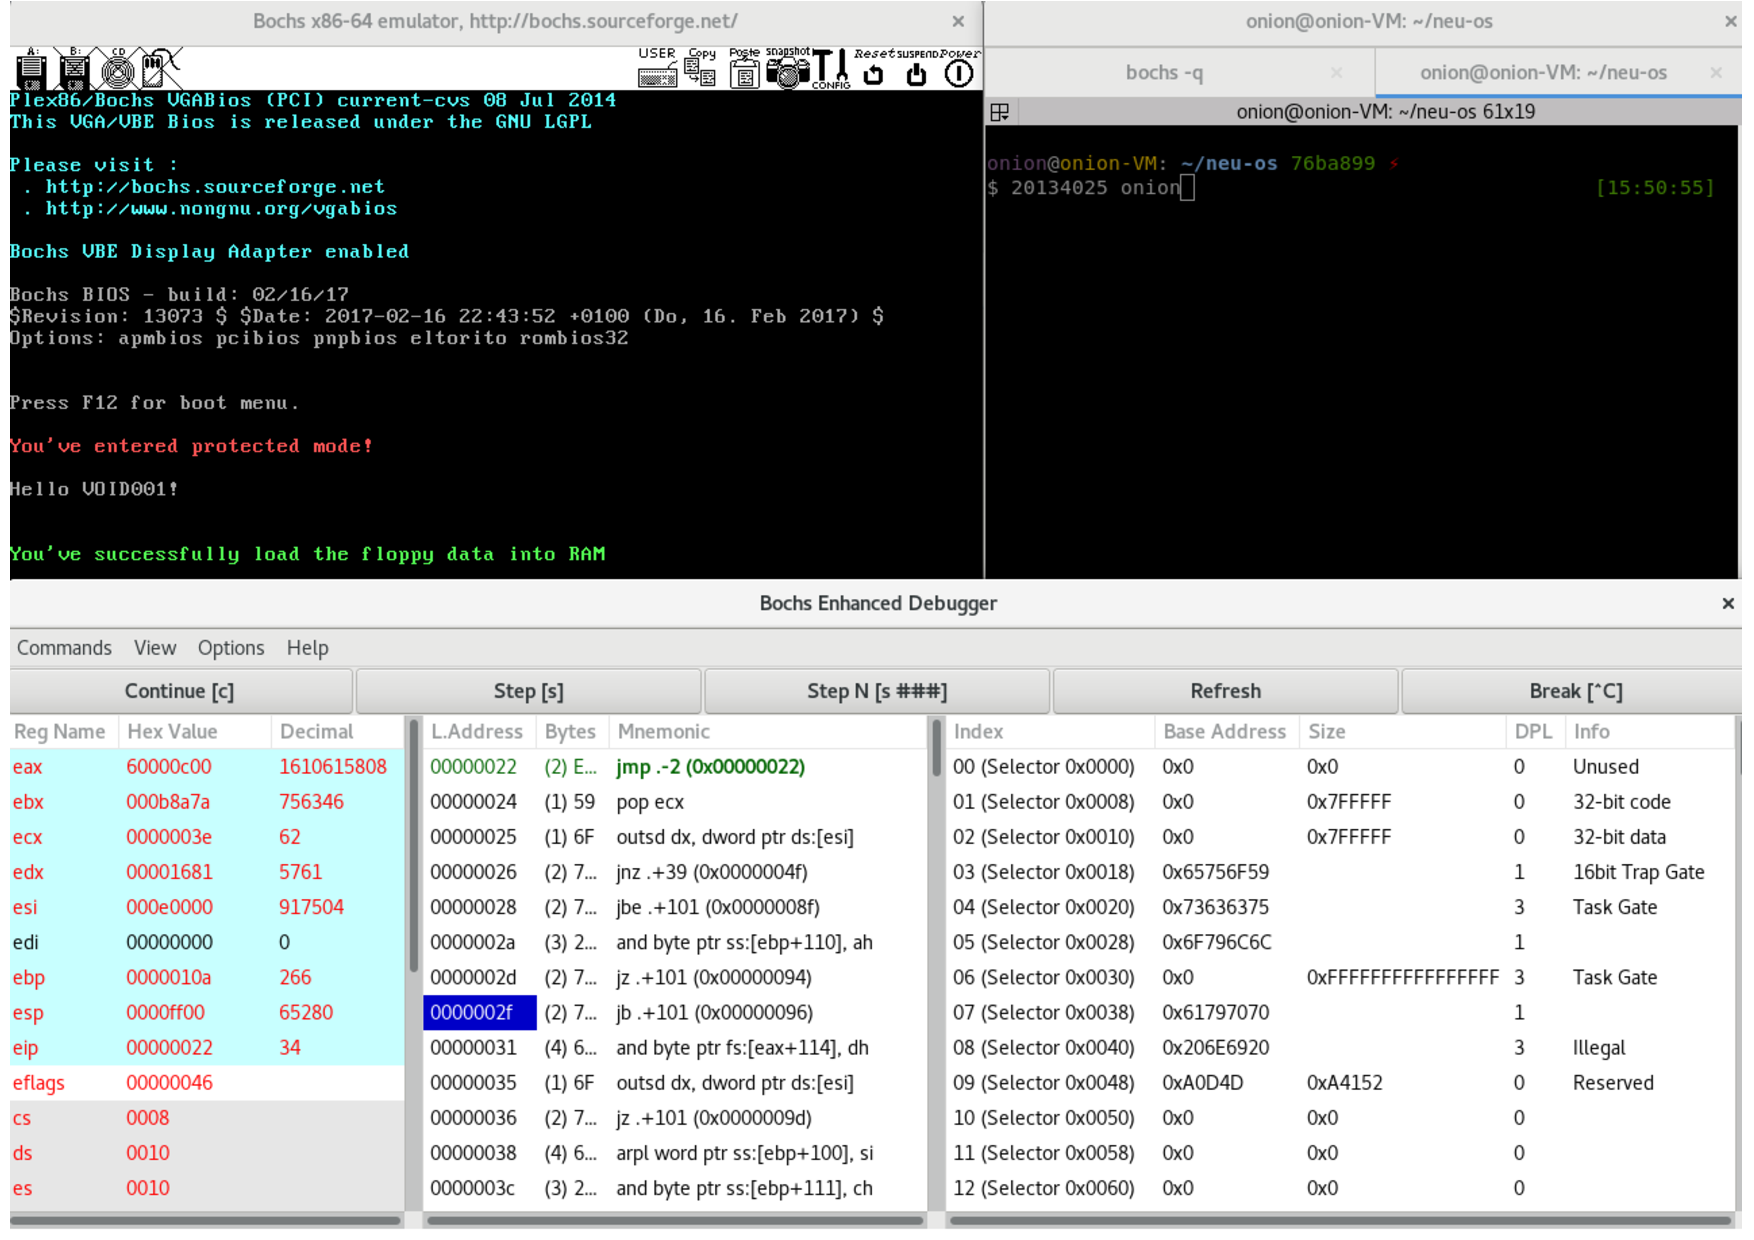
\includegraphics[width=\textwidth]{img/Bochs查看GDT.pdf}
    \caption{Bochs 查看 GDT}
    \label{fig:Bochs查看GDT}
\end{figure}

\subsection{保护模式下的特权级}

保护模式下特权级有 4 种,权限由高到低编号为 0-3。Linux 仅使用了 0 号和 3 号,它们分别是内核态和用户态。

% 参考文档
\begin{itemize}
    \item INT table:\url{http://stanislavs.org/helppc/int_table.html} 用于查询 int 中断用法。
    \item 本次实验视频教程:\url{https://www.bilibili.com/video/av13053659/}
    \item Intel® 64 and IA-32 Architectures Software Developer’s Manual:\url{https://software.intel.com/sites/default/files/managed/39/c5/325462-sdm-vol-1-2abcd-3abcd.pdf}
\end{itemize}

\begin{mdframed}[hidealllines=true,backgroundcolor=gray!20]
\textbf{拓展学习 }
[从零开始的操作系统编写 Lesson 0x01] \url{ https://www.bilibili.com/video/av12367780/?t=1945}
\end{mdframed}

\begin{mdframed}[hidealllines=true,backgroundcolor=gray!20]
\textbf{拓展学习 }编写 Linker Script:
打开 exp2/ld-bootsect.ld,尝试为 bootsect.s
编写链接脚本。建议参考上述视频。
\end{mdframed}